%%%%%%%%%%%%%%%%%%%%%%%%%%%%%%%%%%%%%%%%%%%%%%%%%%%%%%%%%%%%%%%%%%%%%%%%%%%%%%
\section{Evaluation}\label{sec:evaluation}
%%%%%%%%%%%%%%%%%%%%%%%%%%%%%%%%%%%%%%%%%%%%%%%%%%%%%%%%%%%%%%%%%%%%%%%%%%%%%%

We implemented our approach as a plugin for Borealis bounded model checker and conducted some preliminary evaluation. We interested in three kinds of results: number of finding bugs and time of analyzing. We launched the project in 3 modes: with approximation, without interprocedural analysis and with inlining.

We selected five~C~projects of different size and complexity for our evaluation: \texttt{Silver_search}, \texttt{Glove}, \texttt{C4}, \texttt{KSCP} and \texttt{Progress}. The evaluation results are shown in table~\ref{table:evaluation}.

\begin{table}[H]
\centering
\caption{Evaluation results}
\label{table:evaluation}
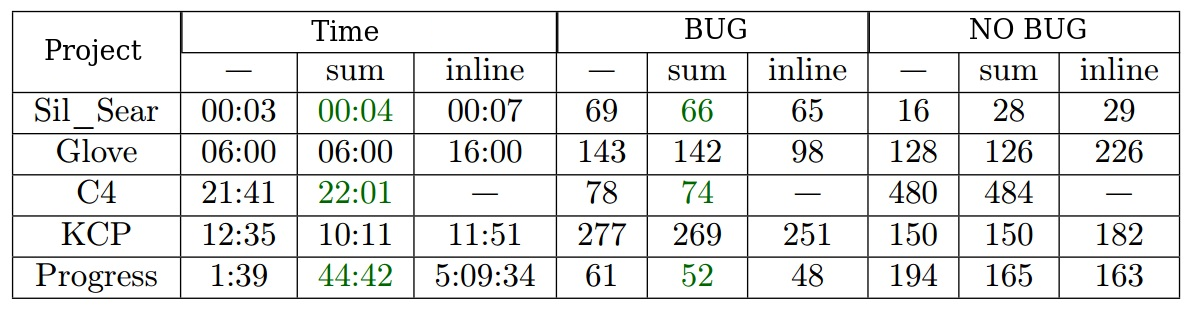
\includegraphics[keepaspectratio, width=\linewidth, height=8cm]{testing}
\end{table}

Testing can be considered successful if results in approximation mode are close to results in inlining mode and time in approximation mode is less than in inlining mode. We can see from table~\ref{table:evaluation} that the results are dependent on the analyzing project. If a project does not contain functions, which assign a return value to constant, we can not approximate them, and results such as without interprocedural analysis~(e.g., \texttt{Glove}). In others projects our algorithm shows positive influence on the analysis process. 
